\documentclass[a4paper,12pt]{article}
\usepackage{geometry}
\usepackage{wrapfig}
\geometry{
	a4paper,
	total={170mm,257mm},
	left=10mm,
	right=10mm,
	top=20mm,
}
\usepackage{titlesec}
\titlelabel{\thetitle.\quad} %точка в section

%%% Работа с русским языком
\usepackage{cmap}                           % поиск в PDF
\usepackage{mathtext} 			 	       % русские буквы в формулах
\usepackage[T2A]{fontenc}               % кодировка
\usepackage[utf8]{inputenc}              % кодировка исходного текста
\usepackage[english,russian]{babel}  % локализация и переносы

%Математика
\usepackage{amsmath,amsfonts,amssymb,amsthm,mathtools} % AMS
\usepackage{icomma} % "Умная" запятая

%% Шрифты
\usepackage{euscript}	 % Шрифт Евклид
\usepackage{mathrsfs} % Красивый матшрифт

\usepackage{gensymb}
\usepackage{graphicx}
\usepackage{setspace}
\usepackage{tabularx}
\usepackage{longtable}
\usepackage{icomma}
\usepackage{euscript}
\usepackage{float}
\usepackage{cutwin}
\usepackage{adjustbox}
\usepackage{dashbox}
\usepackage[normalem]{ulem}
\usepackage[babel=true]{microtype}
\RequirePackage[T1]{fontenc}
\usepackage{amsmath,amsfonts,amssymb,amsthm,mathrsfs,mathtools}
\usepackage{xcolor}
\usepackage{enumitem}
\usepackage{xpatch}
\usepackage{cancel}
\usepackage{upgreek}
\usepackage{lipsum}
\usepackage[version=4]{mhchem}
\usepackage{multirow}
\usepackage{stackengine}
\usepackage{tikz}
\usepackage{hyperref}
\hypersetup{colorlinks=true,urlcolor=blue}
\usetikzlibrary{positioning}
\usepackage{titletoc}
\usepackage{chngcntr}
\usepackage{fancyhdr}
\usepackage{makecell}
\usepackage{indentfirst}
\usepackage{tocloft}
\usepackage{soul}
\usepackage[stable]{footmisc}
\usepackage{subfig}
\usepackage{comment}


\mathtoolsset{showonlyrefs=true}


\theoremstyle{definition}
\newtheorem*{definition}{Определение}
\newtheorem{statement}{Предложение}[section]
\newtheorem{lemma}{Лемма}[section]
\newtheorem{theorem}{Теорема}[section]
\newtheorem*{theoremn}{Теорема}
\newtheorem*{corollary}{Следствие}
\newtheorem*{example}{Пример}
\newtheorem*{note}{Замечание}
\newtheorem*{problem}{Задача}


\counterwithout{footnote}{section}\DeclareRobustCommand{\divby}{%
	\mathrel{\text{\vbox{\baselineskip.65ex\lineskiplimit0pt\hbox{.}\hbox{.}\hbox{.}}}}%
}

\newcommand{\dotpr}[2]{\bra{#1}\ket{#2}}
\let\AA\relax
\let\emptyset\varnothing
\DeclareMathOperator*{\esssup}{ess sup}
\DeclareMathOperator*{\ord}{ord}
\DeclareMathOperator*{\supp}{supp}
\DeclareMathOperator*{\pr}{pr}
\DeclareMathOperator*{\Ker}{Ker}
\DeclareMathOperator*{\Vol}{Vol}
\DeclareMathOperator*{\rg}{rk}
\DeclareMathOperator*{\Ima}{Im}
\DeclareMathOperator*{\Alt}{Alt}
\DeclareMathOperator*{\Sym}{Sym}
\newcommand{\eqdef}{\stackrel{\text{\tiny{def}}}{=}}
\newcommand{\pp}{\partial}
\newcommand{\AA}{\mathcal{A}}
\newcommand{\BB}{\mathcal{B}}
\newcommand{\MM}{\mathbb{M}}
\newcommand{\NN}{\mathbb{N}}
\newcommand{\ZZ}{\mathbb{Z}}
\newcommand{\QQ}{\mathbb{Q}}
\newcommand{\RR}{\mathbb{R}}
\newcommand{\CC}{\mathbb{C}}
\newcommand{\FFF}{\mathbb{F}}
\newcommand{\DD}{\mathcal{D}}
\newcommand{\FF}{\mathcal{F}}
\newcommand{\sS}{\mathcal{S}}
\newcommand*\circled[1]{\tikz[baseline=(char.base)]{
		\node[shape=circle,draw,inner sep=2pt] (char) {#1};}}

%%% Заголовок
\author{Балдин Виктор Б01-303}
\title{Лабораторная работа 4.1.1 \\
	\textbf{Геометрическая оптика}}
\date{\today}

\begin{document}

{\Large \maketitle}

	\paragraph*{Цель работы:} изучение свойств оптических систем: определение фокусных расстояний линз, определение фокусных расстояний и положения главной и фокальной плоскостей сложной оптической системы, изучение аббераций оптических систем.

	\paragraph*{В работе используются:} оптическая скамья с набором рейтеров, положительные и отрицательные линзы, экран, осветитель с ирисовой диафрагмой, зрительная труба, кольцевые диафргамы, линейка.

\section{Введение}
\subsection*{Определения фокусных расстояний}
Формула тонкой линзы имеет вид
\begin{equation}
    \frac{1}{f} = \frac{1}{a} + \frac{1}{b},
\end{equation}
\noindent
где $f$ -- фокусное расстояние, $a$ -- расстояния от предмета до линзы, $b$ -- расстояние от изображения до линзы.

\noindent
Для измерения фокусного расстояния тонкой собирающей линзы может использоваться схема с рис. 1. и формула (2).
\begin{equation}
    f = \frac{L^2 - l^2}{4L}
\end{equation}

\begin{figure}[H]
    \centering
    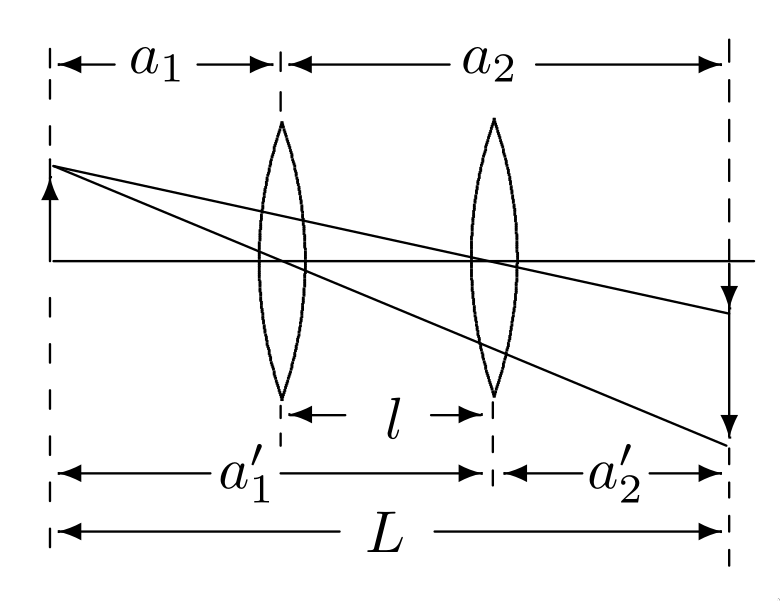
\includegraphics[scale=0.3]{pic_1.png}
    \caption{Схема измерения фокуса тонкой собирающей линзы}
\end{figure}

\noindent
Также фокусное расстояние тонкой собирабщей линзы можно измерить с помощью зрительной трубы, настроенной на бесконечность. Если расположить линзу между предметом и трубой и найти четкое изображение предмета, то расстояние от линзы до предмета будет равно фокусному.

\noindent
Для определения расстояние тонкой рассеивающей линзы поспользуемся схемой на рис. 2 и формулой тонкой линзы. Также можно восползоваться зриетльной трубой, настроенной на бесконечность. Если расположить предмет у нее в фокусе, то изображение переместиться в бесконечность, что можно проверить с помощью зрительной трубы.

\begin{figure}[H]
    \centering
    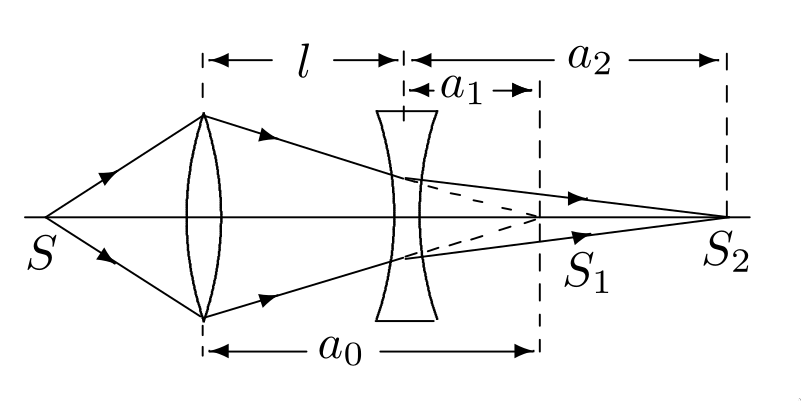
\includegraphics[scale=0.35]{pic_2.png}
    \caption{Схема измерения фокуса тонкой рассеивающей линзы}
\end{figure}

\noindent
Для определения фокусного расстояние и положения главных плоскостей сложной оптической системы может использоваться метод Аббе: схема на рис. 3 и формула (3).

\begin{figure}[H]
    \centering
    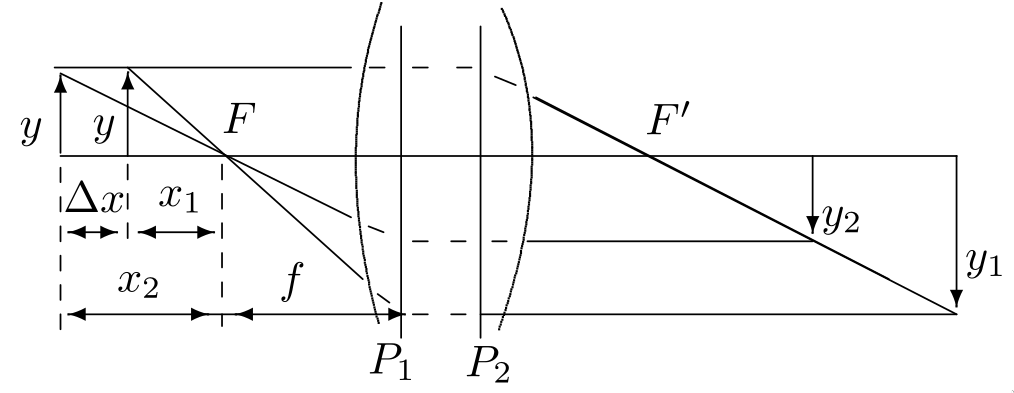
\includegraphics[scale=0.3]{pic_3.png}
    \caption{Схема определения фокусного расстояние и положения главных плоскостей сложной оптической}
\end{figure}

\begin{equation}
    f = \frac{\Delta x}{y / y_1 - y / y_2}
\end{equation}

Пусть пучок света, попадающий в объектив, составляет с оптической осью угол $\varphi_1$, а пучок, выходящий из окуляра, — угол $\varphi_2$. Увеличение $\gamma$ зрительной трубы по определению равно
\begin{equation}
    \gamma = \frac{\tan \varphi_2}{\tan \varphi_1},
\end{equation}
но также из рис. 3 следует, что
\begin{equation}
    \gamma_K = \frac{f_1}{f_2} = \frac{D_1}{D_2},
\end{equation}
где $D_1$ - ширина пучка, прошедшего через объектив, а $D_2$ - ширина пучка, вышедшего из окуляра

\subsection{Моделирование трубы Галилея}

    \begin{figure}[H]
    \centering
    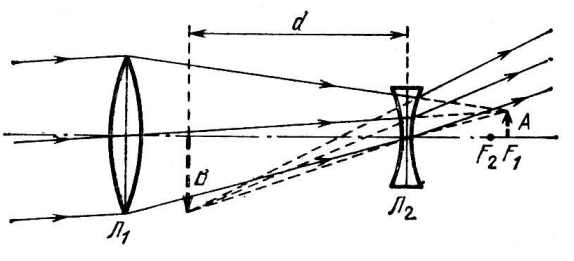
\includegraphics[width=9cm]{gal.PNG}
    \caption{Ход лучей в трубе Галилея}
    \label{fig:vac}
\end{figure}

\subsection{Моделирование микроскопа}

    \begin{figure}[h]
    \centering
    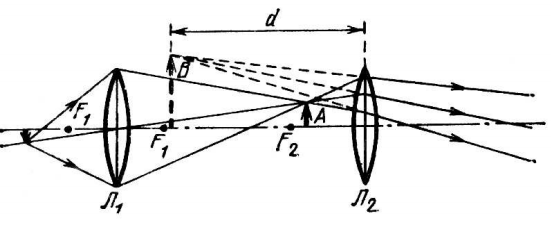
\includegraphics[width=9cm]{micro.PNG}
    \caption{Ход лучей в микроскопе}
    \label{fig:vac}
\end{figure}


Ход лучей в микроскопе показан на рис. 6. Увеличение микроскопа вычисляется по формуле
    \begin{equation}
        \gamma_M = \Gamma_{o_b} \Gamma_{o_c} = \frac{\triangle}{f_1} \frac{L}{f_2},
    \end{equation}.

    \begin{figure}[h]
    \centering
    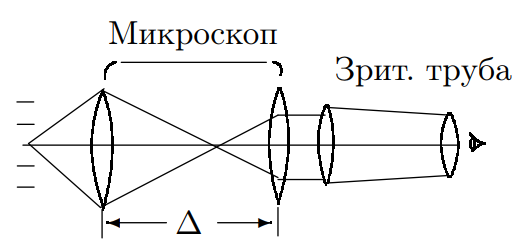
\includegraphics[width=9cm]{micro_2.PNG}
    \caption{Схема микроскопа}
    \label{fig:vac}
\end{figure}


\newpage
% \section{Ход работы}
% \subsection{Подготовка к работе}
% %\par Работал я за установкой №3. Визуально определим, какие линзы являются собирающими, а какие -- рассеивающими. Собирающие линзы: 1, 2, 3, 4; рассеивающая линза: 5. Откорректируем высоту линз. Линза 1 не опускается ниже определённого уровня, так что использовать её далее мы не будем.
% \par Определим фокусные расстояния линз с помощью экрана. С помощью формулы тонкой линзы подбирая расстояния между экраном, линзой и источникм, находим оценочные фокусные расстояния линз. Для нахождения фокусного расстояния рассеивающей линзы, поставим вплотную к ней собирающую, оптическая сила будет суммой сил каждой из линз. Тогда получаем

% \begin{table}[h!]
% \centering
% \begin{tabular}{|l|l|l|l|}
% \hline
% $F_2$, см  & $F_3$, см & $F_4$, см  & $F_5$, см  \\ \hline
% 16 & 20 & 30 & -10 \\ \hline
% \end{tabular}
% \end{table}

% \subsection{ Определение фокусных расстояний линз с помощью зрительной трубы}

% Так как мы настроили зрительную трубу на бесконечность, то, если линза будет находится ровно на фокусном расстоянии от источника, то глядя в трубу мы будем видеть четкое изображение.

% Для нахождения фокусного расстояние отрицательной линзы так же воспользуемся вспомогательной положительной, создавая для отрицательной линзы мнимый источник. Тогда фокусное расстояние отрицательной линзы будет $f = a_0 - l$


% \begin{figure}[h]
%     \centering
%     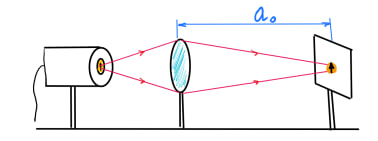
\includegraphics[width=9cm]{d1.jpg}
%     \label{fig:vac}
% \end{figure}

% \begin{figure}[h!]
%     \centering
%     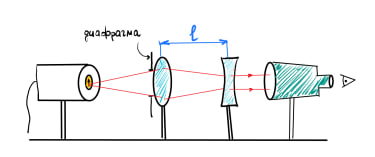
\includegraphics[width=9cm]{d2.jpg}
%     \label{fig:vac}
% \end{figure}

\section*{Ход работы}
\subsection*{Определения фокусных расстояний}
\paragraph{Юстировка} сначала разделим имеющийся набор на собирающие и рассеивающие линзы и отцентрируем установку. Собирающие линзы: 1, 2, 3; рассеивающие линзы: 4.

\paragraph{Определение фокусных расстояний линз с помощью экрана}
Воспользуемся сначала схемой на рис. 1 и формулой (2) для определения фокусного расстояния линзы 1. При измерении расстояний получаем $L = 48.0 \pm 0.2$ см, $l = 25.1 \ pm 0.2$ см. Отсюда ее фокусное расстояние $f = 8.7 \pm 0.3$ см. \\
Также мы можем воспользоваться формулой тонкой линзы для определения фокусного расстояния: $a = 31.0 \pm 0.3$, $b = 14.0 \pm 0.3$. Тогда $f = 10.0 \pm 0.5$ см. \\
Теперь воспользуемся схемой на рис. 2 и формулой тонкой линзы для определения фокусного расстояния рассеивающей линзы 4: $a_0 = 31 \pm 0.3$ см, $l = 24.2 \pm 0.3$ см, $a_2 = 17.5$ см. Отсюда $f = 8.5 \pm 4$ см.

\paragraph{Определение фокусных расстояний линз с помощью зрительной трубы}
Фокусные расстояния, определенные с помощью зрительной трубы, составляют
\begin{itemize}
    \item для линзы 1 $f = 10.5 \pm 0.3$ см, что существенно отличается от значения $f = 8.7 \pm 0.3$ см, полученного ранее, поэтому линзу нельзя считать тонкой.
    \item для линзы 2 $f = 13.4 \pm 0.3$ см.
    \item для линзы 4 $f = 9.0 \pm 0.4$ см.
\end{itemize}

\paragraph{Определение фокусного расстояния сложной оптической системы} воспользуемся схемой на рис. 3 и формулой (3) для определения фокусного расстояния и положения главных плоскостей системы методом Аббе. Для этого сначала соберем установку согласно рис. 3, расположив линзы 1 и 2 на расстоянии  на расстоянии $l_{12} = 30$ см друг от друга. Измерив необходимые расстояния, получаем: $\Delta x = 2.4 \pm 0.3$ см, $y_1 = 5.1 \pm 0.1$ см, $y_2 = 12.3 \pm 0.1$ см, $y = 2.0$ см. Отсюда фокусное расстояние системы $f = 10.5 \pm 0.5$ см. С помощью зрительной трубы найдем главные фокусы системы: для этого закрепим трубу за второй линзой и будем отодвигать источник, пока не увидим четкое изображение. Для определения второго фокуса поменяем линзы местами, не меняя расстояний в системе. Полученные значения главынх фокусов $F_{1\Sigma} = 5.1 \pm 0.3$ см, $F_{2\Sigma} = 4.5 \pm 0.3$ см.

\subsection*{Аберрации реальных оптических систем}
\paragraph{Сферические аберрации} для качетсвенного наблюдения сферических аберраций расположим осветитель и экран на дальних концах скамьи. Линзу 3 расположим на расстоянии чуть большем фокусного от источника. На источник наденем маску минимального размера. Перемещая линзу, получим на экране четкое изображение. При смеге маски наблюдаем, что пр неизменном расстоянии от источника до линзы расстояние от линзы до изображения заметно меняется. Это объясняется сферической аберрацией. \\
Для количественной оценки сферической аберрации сначала получим параллельный пучок от линзы для параксиальных лучей. Затем, увеличиваю диаметр маски, будем менять положение линзы с помощью нониусного винта и измерять расстояния по нониусной шкале $d$. Резульаты измерений представлены в табл. 1. Погрешность измерения $d$ составляет $0.1$ мм.

\begin{table}[H]
    \centering
    \caption{Сферические абберации}
    \begin{tabular}{|c|c|c|c|} \hline
        $h$, мм & 0 & 5 & 20 \\ \hline
        $d$, мм & 0 & 0.8 & 2.9 \\ \hline
    \end{tabular}
\end{table}

\noindent
По результатм этих измерений построим зависимость $\delta s(h)$, представленную на рис. 4. Эксраполируя эту зависимость до $h = r$, где $r$ -- радиус линзы, найдем продольную аберрацию $\delta s(r) = \Delta f(r) = 3.6$ мм.

\begin{figure}[H]
    \centering
    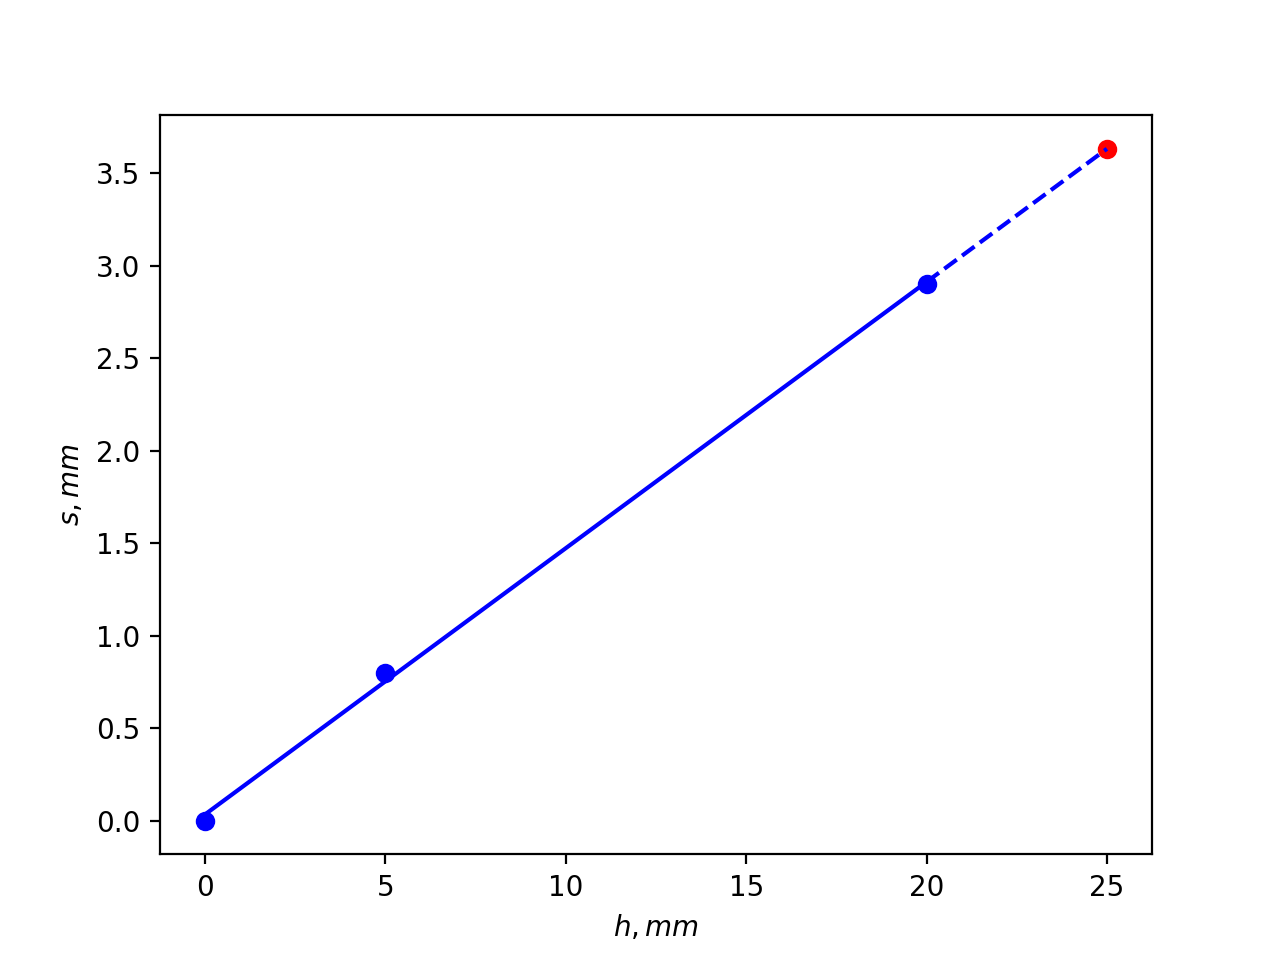
\includegraphics[scale=0.9]{1.png}
    \caption{Сферические аберрации}
\end{figure}

\newpage
\paragraph{Хроматические аберрации} пользуясь тремя светофильтрами, найдем значения $f_D = 13.5$ мм, $f_F = 13.9$ мм, $f_C = 13,3$ мм. Отсюда, пользуясь формулами (5) и (7), находим $\nu \approx 23$, $\delta f_\text{хр} = 0.6$ мм.


\section*{Вывод}
Мы измерили фокусные расстояния нескольких линз, а также системы линз. Получены значения:
\begin{itemize}
    \item для линзы 1 фокусное расстояние $f = 10.5 \pm 0.3$ cм, линзу нельзя считать тонкой
    \item для линзы 2 фокусное расстояние $f = 13.4 \pm 0.3$ см
    \item для линзы 4 фокусное расстояние $f = 9.0 \pm 0.4$ см при измерении с помощью трубы, $f = 8.5 \pm 0.4$ см при измерении с помощью экрана. Линзу можно считать тонкой
    \item для системы из линз 1 и 2 фокусное расстояние состаляет $f = 10.5 \pm 0.5$ см, положения главынх фокусов $F_{1\Sigma} = 5.1 \pm 0.3$ см, $F_{2\Sigma} = 4.5 \pm 0.3$ см
\end{itemize}
Также качественно пронаблюдали и оценили сферические и хроматические абберации. Получены значения продольной сферической аберрации $\delta s(r) = 3.6$ мм и хроматической аберрации $\delta f_\text{хр} = 0.6$ мм, а также оценено число Аббе $\nu \approx 23$.


\end{document}




\end{document}